\documentclass[a4paper]{article}

% \usepackage[german]{babel}

\usepackage{enumitem}
\usepackage{tikz}
\usepackage{longtable,environ,threeparttablex} 
\usepackage{amssymb,amstext,pdflscape,fancyhdr,threeparttable,verbatim} 
\usepackage[fleqn]{amsmath}
\usepackage{listings}
\usepackage{natbib}
\usepackage[labelsep=space]{caption}
\usepackage{placeins}
\usepackage{float}
\usepackage{subfig,graphicx}

%\usepackage{stmaryrd} - St Mary Road symbols for theoretical computer science
% \usepackage{graphicx} %- zur Einbindung von Bildern
\graphicspath{ {./images/} }
%\usepackage{wrapfig} - um Tabellen und Bilder von Schrift umfliessen zu lassen
%\usepackage{tikz} - zur Erstellung von Vektorgrafiken
\usepackage{geometry}
\geometry{
  left=2cm,
  right=2cm,
  top=3cm,
  bottom=4cm,
  bindingoffset=5mm
}
\usepackage{setspace}
\usepackage{textpos}

\makeatletter
\newcommand{\MSonehalfspacing}{%
  \setstretch{1.44}%  default
  \ifcase \@ptsize \relax % 10pt
    \setstretch {1.448}%
  \or % 11pt
    \setstretch {1.399}%
  \or % 12pt
    \setstretch {1.433}%
  \fi
}
\newcommand{\MSdoublespacing}{%
  \setstretch {1.92}%  default
  \ifcase \@ptsize \relax % 10pt
    \setstretch {1.936}%
  \or % 11pt
    \setstretch {1.866}%
  \or % 12pt
    \setstretch {1.902}%
  \fi
}
\makeatother
\MSonehalfspacing


%%%%%%%%%%%%%%%%%%%%%%% Defining head %%%%%%%%%%%%%%%%%%%%%%%%%%%%%%%%
\pagestyle{fancy}
\fancyhf{} % alle Kopf- und Fußzeilenfelder bereinigen
\fancyhead[L]{Department of Political Science and Public Administration \\ Prof. Dr. Susumu Shikano}
\fancyhead[R]{University of Konstanz} 
\renewcommand{\headrulewidth}{0.5pt} %obere trennlinie
\fancyfoot[C]{\thepage} %Seitennummer
%\renewcommand{\footrulewidth}{0.4pt} %untere trennlinie


\begin{document}

\begin{center}  	
\Large{Research Proposal}\\
\today
\vspace{1cm}
\end{center}

%%%%%%%%%%%%%%%%%%% Start Document here %%%%%%%%%%%%%%%%%%%%%%

\begin{textblock*}{\textwidth}(0cm,-0.5cm)
    \textbf{Student Name:} Rahkakavee Baskaran

    \textbf{Supervisor:} Prof. Dr. Susumu Shikano

    \textbf{Supervisor:} JunProf. Dr. Juhi Kuleshtra

\end{textblock*}

\medskip

\medskip

\section{Introduction}
Job titles are key information within the labor market. They are useful for job seekers to find jobs \citep{Marinescu2020}. They are an important component of job search engines \citep{Slamet018, Javed2015, Javed2016} and job recommendation systems \citep{Malherbe2014}. And lastly, they serve as a valuable data source for various analyses, such as job market trend \citep{Martin2021, Li2021}, job perception \citep{Smith1989, Bodyston2019} or social science analyses \citep{Martin2021}. However, since job titles are not normalized, it is challenging to structure them in an appropriate way for downstream tasks. Various institutions developed job taxonomies in order to structure and generalize job titles. Established taxonomies are, for example, the ``International Standard Classification of Occupation'' (ISCO) for the European job market or the ``Klassifikation der Berufe 2010'' (KLdB) for the German job market \citep{Uter2020}. Matching job titles from job postings with classes from those taxonomies is inevitable in order to improve job search engines or recommendation systems as well as analyzing the labor market. In Natural Language Processing (NLP), this process of matching is known as text classification. 

Text classification, a highly researched area, is the process of classifying text documents or text segments into a set of predefined classes. During the last decades, researches developed a various number of classifiers. As \cite{Kowsari2019} summarize in their survey of classifiers, we can group the approaches mainly into three groups. The first group contains traditional methods like Naive Bayes (NV), Support Vector Machines (SVM), K-nearest neighbors (KNN),  Logistic Regressions (LR) or Decision Trees (DT) \citep{Vijayan2017, Colas2006, Kowsari2019, Sebastiani2001}. Deep learning methods like Convolutional Neural Networks (CNN) or Recurrent Neural Networks (RNN), which are currently the most advanced algorithms for NLP, form the second group. The last group consists of ensemble learning techniques like Boosting and Bagging.

Each text classification task presents different challenges. One challenge is that domain-specific problems may arise. There is some work that deals with job classification in the English speaking job market. 
In terms of classifiers, the corresponding work can be categorised into traditional classifiers or deep learning methods. \cite{Zhu2017} for example, use a KNN classifier in combination with document embedding as feature selection strategy. \cite{Javed2015} rely on traditional methods as well, by combining a SVM classifier and a KNN classifier for their job recommendation system. In contrast, the approaches of \cite{Decorte2021}, \cite{WangJ2019} and \cite{Neculoiu2016} are based on Deep Learning methods. From a higher perspective, there is another dividing line between the approaches. As mentioned earlier, job title normalization can be considered as a typical text classification task \citep{WangJ2019, Javed2015, Zhu2017}. \cite{Decorte2021} and \cite{Neculoiu2016}, however, formulate the task as a string representation approach of similar job titles.  

Another potential issue is the length of input documents for classification. Job titles are clearly short text with often not more than 50 characters. Short texts suffer from sparseness, few word co-occurrences, missing shared context, noisiness and ambiguity. Traditional methods, however, are based on word frequency, high word co-occurrence and context, which is why they often fail to achieve high accuracy for short texts \citep{Song2014, WangY2017, WangF2014}. In their overview, \cite{Song2014} present three approaches to solve this. First, since short text data often suffers from unlabeled data in the context of online text data, such as Twitter postings, they suggest using semi-supervised approaches. Second, they recommend to use ensemble learning methods, which focus on the sparseness of the data. Third, \cite{Song2014} propose feature dimensionality reduction and extraction of semantic relationship methods. Based on the latter more recent work on short text classification criticizes the use of the ``Bag of Word'' concept for feature representation as it only reflects the appearance of words in the text. Instead, they represent short texts with semantically similar and conceptual information \citep{Bouaziz2014, WangF2014, Chen2019}.
Another question concerning the representation of short texts is whether to represent them as dense or sparse vectors. In their comparison between tf-idf/counter vectorizer and the dense vectorizer word2vec and doc2vec, \cite{WangY2017} conclude that among the classifiers Naive Bayes, Logisitic Regression and SVM, the sparse vectorizers achieve the highest accuracy. \cite{Chen2019}, conversely, see limitations in sparse representation as it cannot capture the context information. In their work, they integrate sparse and dense representation into a deep neural network with Knowledge powered Attention, which outperform state-of-art deep learning methods, like CNN, for Chinese short texts. 
Concerning the classifiers, there is no consensus approach for short text classification. For traditional approaches \cite{WangY2017}'s results indicate that logistic regression and SVM perform best, while KNN seems to achieve best accuracy in \cite{Khamar2013}'s work. Similar to job title specific work, more recent work prefers deep learning methods, mostly CNN \citep{Chen2019}. 

A last challenge of text classification tasks comes with the number of classes. As \cite{Li2004} show in their classification of tissue, multiclass classification is more difficult than binary classification problems. Partly, because most of classification algorithms were designed for binary problems \citep{Aly2005}. Approaches for multiclassification can be grouped into two types. Binary algorithms can handle multiclassification naturally. This is, for example, the case for Regression, DT, SVM, KNN and NV. The second type is the decomposition of the problem into binary classification tasks (for the different subtypes see \cite{Aly2005}). The literature so far does not have a clear answer to solve multiclassification problems. Different approaches, like Boosting \citep{Schapire2000} or CNN \citep{Farooq2017} are applied. It is noticeable, however, that many works use variations of SVM \citep{Guo2015,Tomar2015,Tang2019}. 


\section{Goal of the Thesis}
\subsection{Problem Statement}
The presented work on job classification has several gaps. First, while there is extensive work on job title classification for the English speaking job market, as far as I know, there have not been any classification attempts for the German job market. However, an accurate classification of job titles with the German taxonomy would facilitate several downstream tasks for the German job market. With the KldB 2010, an occupational classification was created for Germany that reflects the current trends in the labor market based on empirical and theoretical foundations. It contains 5 hierarchical levels, each of them reflecting different aspects. Especially level 3, which represents the professionalism of occupations, and level 5, which gives information on the requirements for a job are powerful tools for job market analyses \citep{Paulus2013}. In addition, the KldB 2010 is based on ISCO, which makes it easier to link the two taxonomies. The strengths of the KldB clearly show that an accurate classification of job titles according to KldB 2010 opens up new possibilities for labor market analyses. Furthermore, the classification could improve job search engines and recommendation systems. 

Second, the brevity of the input texts and the large number of classes are the main challenges in job title classification. In the previous approaches to job title classification, the challenges are partly mentioned and considered, but the frameworks are not built on the basis of these challenges. A clear focus on methods from the two problem areas, could help to improve classification.  

Finally, most of the work about job title classification suffers from solid databases. Therefore, \cite{Decorte2021}, for example, use skills to understand the meaning of job titles and to avoid manually labelling them. \cite{Javed2015} rely on a weakly supervised approach to get enough labelled data. The advantage of classifying for the German job market is that the Federal Employment Agency of Germany provides a data set with job titles and the possibility of linking them with die KldB classes, which offers a huge and powerful training data set which in turn allows for more flexibility in which algorithms are applicable.

\subsection{Research Objectives}
Based on the research gaps of job classification and the relevance of a classification algorithm for the KldB Taxonomy for the German job market, I define the following research objective: 

Develop and implement a classification algorithm based on the challenges of short text and multiclass classification in order to match job titles of German job postings with the Taxonomy KldB 2010. Then, the algorithm should be evaluated against current state-of-the-art methods.

\subsection{Expected Results}
The project shall contribute to improve downstream tasks for the German labor market. The goal of this project is to develop a classification algorithm that assigns job titles from job advertisements to the predefined classes of the KldB 2010 Taxonomy with a high precision and recall. In this way, job titles, originally non-standardized pieces of information, are normalized to job classes, which can then be used for analyses, search engines and recommendation systems. The thesis includes recent studies on short text classification and multi class classification, as well as job title classification approaches. 

\section{Methodology}
In order to reach the goals of this Thesis, several tasks have to be fulfilled. 

\subsection*{First exploration}
In a first exploration, the data should be analysed with a simple algorithm in order to check how they would perform for the classification task. The analysis consists of three steps. In the first step, I look at the first ten main groups from level 1 of KldB 2010. Then, I apply the algorithm to the level 3 class and lastly to the level 5 classes, thereby extending the number of classes. I choose level 1, level 3 and level 5 since they have the most valuable information of all levels. Results with a preliminary training data set show the following results: 


Figure 1 \ref{sub@a}, \ref{sub@b} and \ref{sub@c} show the distribution of the classes for each level. In figure 1a we can see that most of the classes are well balanced. The classes for level 3 and level 5 are not well distributed. Figure 1 \ref{sub@b} and Figure 1 \ref{sub@c} show that the subclasses of class 5 and class 7 are strongly unbalanced. In addition some of the subclasses have only few or no training examples, which is not sufficient for training. Besides, there is no example for class zero. Thus, there is a need to rescrape data for certain classes. 


\begin{figure}\centering
  \subfloat[]{\label{a}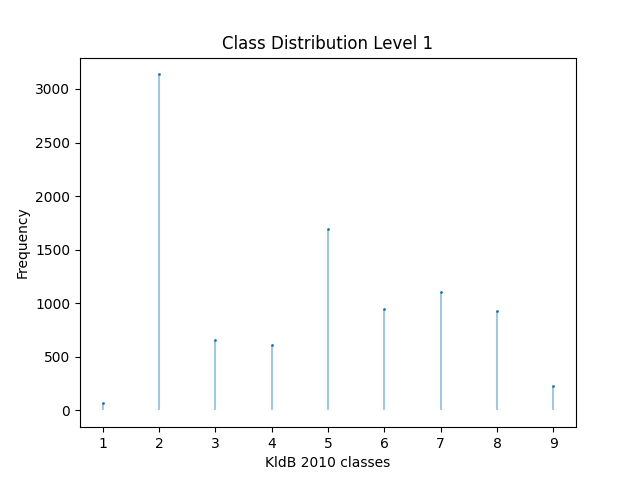
\includegraphics[width=.45\linewidth]{figures/2021-10-22_12-21-00_all_jobs_7_level1.png}}\hfill
  \subfloat[]{\label{b}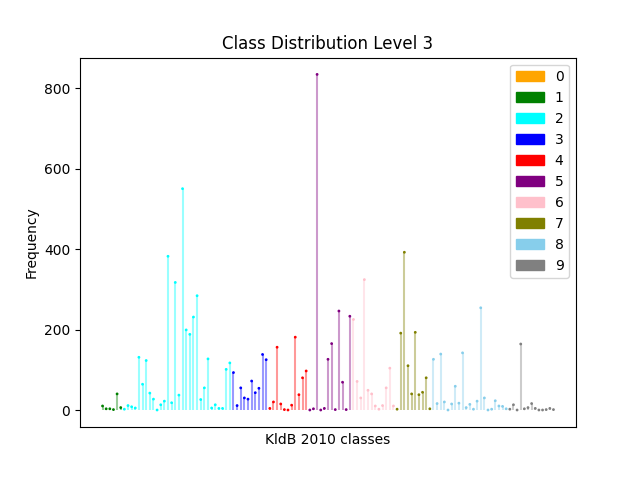
\includegraphics[width=.45\linewidth]{figures/2021-10-22_12-21-00_all_jobs_7_level3.png}}\par 
  \subfloat[]{\label{c}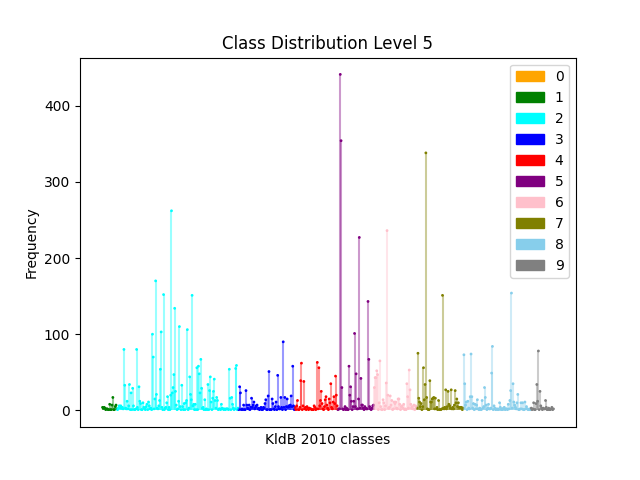
\includegraphics[width=.45\linewidth]{figures/2021-10-22_12-21-00_all_jobs_7_level5.png}}
  \label{fig}
\end{figure}

Table \ref{tab:1} to \ref{tab:3} show the evaluation reports with different classification metrics for the levels 1, 3 and 5. For the first exploration, I used a NB classifier, since it is a quite simple, but usually good performing algorithm. Results indicate for level 1 a moderate precision and recall. With increasing number of classes, precision and recall clearly decrease. 

\begin{table}
  \begin{center}
  \caption{Classification Report Level 1}
  \label{tab:1}
  \begin{tabular}{lrrrr}
    \hline
  {} &  precision &    recall &  f1-score &      support \\ \hline
  1            &   0.050633 &  0.727273 &  0.094675 &    11 \\
  2            &   0.884615 &  0.498724 &  0.637847 &   784\\
  3            &   0.328947 &  0.709220 &  0.449438 &   141\\
  4            &   0.443182 &  0.726708 &  0.550588 &   161\\
  5            &   0.818681 &  0.683486 &  0.745000 &   436 \\
  6            &   0.529801 &  0.730594 &  0.614203 &   219 \\
  7            &   0.813559 &  0.491468 &  0.612766 &   293 \\
  8            &   0.809091 &  0.744770 &  0.775599 &   239\\
  9            &   0.336283 &  0.633333 &  0.439306 &    60\\
  macro avg    &   0.557199 &  0.660620 &  0.546603 &  2344 \\
  weighted avg &   0.740923 &  0.611775 &  0.641521 &  2344 \\
  \hline
  accuracy     &    &   &       0.611775 & 2344 \\
  \hline
  \end{tabular}
\end{center}
\end{table}


\begin{table}
  \begin{center}
    \label{tab:2}
  \caption{Classification Report Level 3}
  \begin{tabular}{lrrrr}
    \hline
    {} &  precision &    recall &  f1-score &      support \\
    \hline
    macro avg    &   0.330428 &  0.399629 &  0.321017 &  2344 \\
    weighted avg &   0.544320 &  0.422782 &  0.446718 &  2344\\
    \hline
    accuracy     &   &  &  0.422782 &     23144 \\
    \hline
    \end{tabular}
  \end{center}
\end{table}

\begin{table}
  \caption{Classification Report Level 5}
  \begin{center}
    \label{tab:3}
\begin{tabular}{lrrrr}
  \hline
  {} &  precision &    recall &  f1-score &      support \\
  \hline
  macro avg    &   0.260878 &  0.282669 &  0.240905 &  2344\\
  weighted avg &   0.474158 &  0.342577 &  0.367748 &  2344\\
  accuracy     &    &   &  0.342577 &     2344\\
  \hline
  \end{tabular}
\end{center}
\end{table}




\subsection*{Training data}
The training data is scraped from the ``Bundesagentur für Arbeit'' (BA), which provides current job postings. The advantage of this data set is, that it is already structured, with each entry containing the job title and the ``Dokumentationskennziffer'' (Dkz). The Dkz is a internal key, which can be easily mapped to the KldB 2010 IDs \citep{Paulus2013}. Hence, the training data can be constructed from BAs structured data, together with the KldB 2010 classes and the job title. 

Most of the classification approaches demand the data to be balanced. In real world application this is often not possible \citep{Japkowicz2000}. Especially for level 5 it is difficult to get enough data for all classes. The descriptive analysis of the first exploration clearly shows that the data is unbalanced for level 3 and level 5, having zero observations in some classes. This has to be handled in some way in the classification process itself or the data must be post-scraped for specific classes. Since the BA updates the data daily, the second way should be enough for most of the classes. In order to do so, I will scrape data regularly to have a solid data base. 

\subsection*{Baseline Algorithms}
The developed algorithm should be compared against the current state-of-the art methods in order to check the improvements. As mentioned in the literature overview, state-of the art methods are Deep Neural Networks, especially CNN. Thus, CNN provides a strong comparison, which is why I will use a simple CNN as the baseline. However, since traditional methods like SVM performed well in some approaches, especially for multi-class handling, it is convenient to also use a traditional approach as baseline. As mentioned in the literature review, often different versions of the SVM algorithm are used. It is therefore a reasonable option to use a basic version of the SVM algorithm. 

\subsection*{Developing of own approach}
As the literature on short text classification shows, the representation of short texts with ``Bag of Words'' is not feasible. Instead, including semantically and conceptual information often leads to better results. The KldB 2010 taxonomy includes for each level 5 class a job description and search words, which allows for the inclusion of a knowledge base into the classification process. In a first step, I will create a knowledge base using the job description and search words. I will use the knowledge base for three approaches. 
In the first approach, I will test the performance of an entity linker, which requires a knowledge base and might already improve the performance. Evaluation will be checked against the named baseline algorithms using precision and recall.

The second approach follows the method of \cite{WangJ2017} by conceptualizing the short text first and then apply a CNN algorithm. 

For the reasons already stated about the baseline algorithms for the SVM classifier, I will also incorporate the knowledge base in an SVM classifier as my third approach. For this, I follow the method suggested by \cite{Le2006}. The advantage of this approach is, that the authors have a specific method for multiclass SVM with knowledge bases. 

After implementing and evaluating these approaches, depending on the results, further improvements or other approaches might be necessary, which will be evident during the development process. 

\section{Timeline}
Each implementation and evaluation step involves taking notes of related literature, theory, implementation steps and results. 
\begin{table}[hb!]
  \begin{tabular}{ll}
  \hline
  \textbf{Date}        & \textbf{Milestone}                                                  \\ \hline
  21 Nov 2021          & Implement baseline algorithms, scrape further data and analyze them \\
  30 Nov 2021          & Implement CNN and entity linker approach and evaluate               \\
  15 Dec 2021          & Implement SVM approach and evaluate                                 \\
  31 Dec 2021          & Write and finish the first version of the MA                        \\
  20 Jan 2022          & Further improvement implementations                                 \\
  31 Jan 2022          & Finish final version of MA                                          \\ \hline
  \textbf{15 Feb 2022} & \textbf{Submission}                                                
  \end{tabular}
  \end{table}

\clearpage

\bibliographystyle{apalike}
\bibliography{export}
    

\end{document}
